\documentclass{../tex_import/ETHuebung_english}

\usepackage{../tex_import/exercise_ml}

\input{../tex_import/definitions} %our customized .tex macros

\begin{document}


\makeheader{4, Oct 2, 2025}{Cross-Validation and Bias-Variance Decomposition}

\paragraph{Goals.}
The goal of this exercise is to
\begin{itemize}
    \item Implement $4$-fold cross-validation.
    \item Understand the bias-variance decomposition.
\end{itemize}

\paragraph{Setup, data and sample code.}
Obtain the folder {\tt labs/ex04} of the course github repository
\begin{center}
\href{https://github.com/epfml/ML\_course/tree/main/labs/ex04}{github.com/epfml/ML\_course}
\end{center}

\section{Cross-validation}

This exercise is partly based on the materials from last week ({\tt labs/ex03}).
If you don't have it already, please finish the ex03 first.
You might directly reuse/copy
some of the functions you implemented yourself during previous exercises,
e.g., {\tt ridge\_regression()}, {\tt least\_squares()} and {\tt build\_poly()}.

% The code structures are as follow:
% \begin{itemize}
% \item biasVariance.py
% \item buildPolynomial.py (from exercise 03)
% \item computeCost.py (from exercise 03)
% \item crossValidationDemo.py
% \item leastSquares.py (from exercise 03)
% \item ridgeRegression.py (from exercise 03)
% \item splitData.py (from exercise 03)
% \end{itemize}


% \section{Cross-Validation}
% % The simple 50\%-50\% split of test and training data from last week's exercise
% % corresponds to the first phase of $2$-fold cross-validation.
% % It may not give an unbiased test error.
% % A better way to do this is to use full $K$-fold cross-validation.

\Exercise{1}{
Implement $4$-fold cross-validation.

\begin{itemize}
\item Copy your code from last week,
and fill in the corresponding templates, i.e.,
{\tt ridge\_regression()} to {\tt ridge\_regression.py},
{\tt build\_poly()} to {\tt build\_polynomial.py},
and {\tt least\_squares()} to {\tt least\_squares.py}.

In this exercise, please fill in the notebook functions {\tt cross\_validation()} and {\tt cross\_validation\_demo()},
and perform $4$-fold cross-validation for polynomial degree $7$.
Plot the train and test RMSE as a function of $\lambda$.
The resulting figure should look like Figure~\ref{fig:cross_validation}.

\item How will you use $4$-fold cross-validation to select the best model among various degrees,
say from 2 to 10? Write code to do it in {\tt best\_degree\_selection()}.

\end{itemize}}

\begin{figure}[!htp]
    \centering
    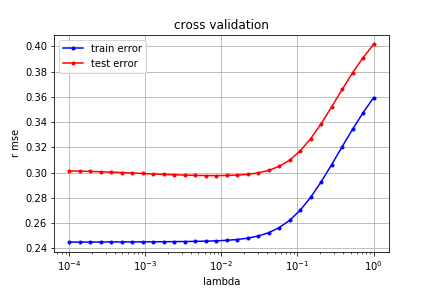
\includegraphics[width=8cm]{solution/cross_validation2.png}\vspace{-2mm}
    \caption{Effect of $\lambda$ on training and test errors,
    calculated using $4$-fold cross-validation}
    \label{fig:cross_validation}
    \end{figure}

\section{Visualizing the Bias-Variance Decomposition}
Last lecture we introduced model selection, and we saw that the model complexity is crucial to the performance. In this problem, we will further investigate the effect of \textit{model complexity} with the concept of \textit{bias-variance decomposition}.
% ML 2021 Fall is quite unusual because the lab is arranged before the second lecture of the week, so I have to introduce all the concepts. Otherwise, un-annotate the following:
% In the lecture, we learned about the expected test and train error.
% In the following exercise, we will reproduce the figure illustrating ``error vs. model complexity'' of the ``bias-variance'' lecture notes).
% Read the lecture notes to understand which quantities are essential for this figure.

We will implement the figures seen in class representing the tradeoff and also seen in Figure ~\ref{fig:bias_variance} : for a big polynomial degree, the bias is small but the variance is large. The opposite is true for a small polynomial degree (however notice that the variance is still quite important). Choosing an intermediate degree leads to consistent predictions which are close to the true function we want to learn (optimal bias / variance tradeoff).

% Consider linear regression with a one-dimensional input and using polynomial feature expansion. The maximum degree $d$ regulates the complexity of the class. Assume that $D$ is the data distribution, and $f_S$ denotes the model trained on the dataset $S$. 

% We will show by experiment that the following is true:

% \begin{itemize}
%     \item Assume that we only allow simple models, i.e., we restrain the degree to be small:
%     \begin{itemize}
%         \item We then typically will get a large bias, i.e., a bad fit.
%         \item On the other hand the variance of $L_D(f_S)$ as a function of the \textit{random} training set $S$ is typically small.
%     \end{itemize}
%     We say that we have high bias but low variance.
%     \item Assume that we allow complex models, i.e., we allow large degrees:
%     \begin{itemize}
%         \item We then typically will find a model that fits the data very well. We will say that we have small bias.
%         \item But we likely observe that the variance of $L_D(f_S)$ as a function of the \textit{random} training set $S$ is large.
%     \end{itemize}
%     We say that we have low bias but high variance.
% \end{itemize}

% Often it is hard to achieve both small bias and variance. This is called \textit{bias-variance trade-off}.

\bigskip

\Exercise{2}{
Visualizing the bias-variance trade-off.
\begin{itemize}
\item
Complete the notebook function {\tt bias\_variance\_one\_seed()}: for $15$ random datapoints, it finds the optimal fit (using the least square formula, with no regularisation $\lambda$) for a polynomial expansion of degree $1$, $3$ and $6$. 
\item you can play around by changing the seed, the number of datapoints, the degree of the polynomial expansion etc.
\item Now complete the notebook function {\tt bias\_variance\_demo()} which performs many times the previous experiment but with a new random training set each time. You should obtain something similar to Figure~\ref{fig:bias_variance}.
\item Comment the figures by explaining how the bias / variance tradeoff is shown in these plots.
\item You can play around by changing the function you want to learn, the variance of the gaussian noise $\sigma^2$, the degree of the polynomial expansion etc.
\item \textbf{BONUS:} you can do similar figures but now you fix the degree of the polynomial expansion and add some regularisation $\lambda$. You will observe a similar bias / variance tradeoff when changing the magnitude of the regularisation.

% \item \textbf{BONUS:} Another good visualization is to use the box-plot to get an appropriate visualization.
% You can clearly see the distribution of test error.


% \item \textbf{BONUS:} Produce the same plot with Ridge regression.
% You will have to automatically find the best $\lambda$ for each degree.
% You do this using $K$-fold cross-validation (CV) only on the training set.
% So you need to insert the CV code inside.
% You also have to make sure that you chose an appropriate range of $\lambda$,
% so that you achieve the minimum test error. What would you expect to happen if you replace least-squares with Ridge regression? Does the experiment result meets your expectation?


%\item \textbf{BONUS:} In the lecture, we discussed that CV produces an estimate of
%expected train and test error. Check if this is the case for this data.
%You can do this using the CV error that you get for Ridge regression
%and then comparing it against the expected test error
%(repeating this for all the training datasets). See Fig.~7.14 of the book by Hastie, Tibshirani, and Friedman.
\end{itemize}
}

% \newpage 



\begin{figure}[!htp]
\centering
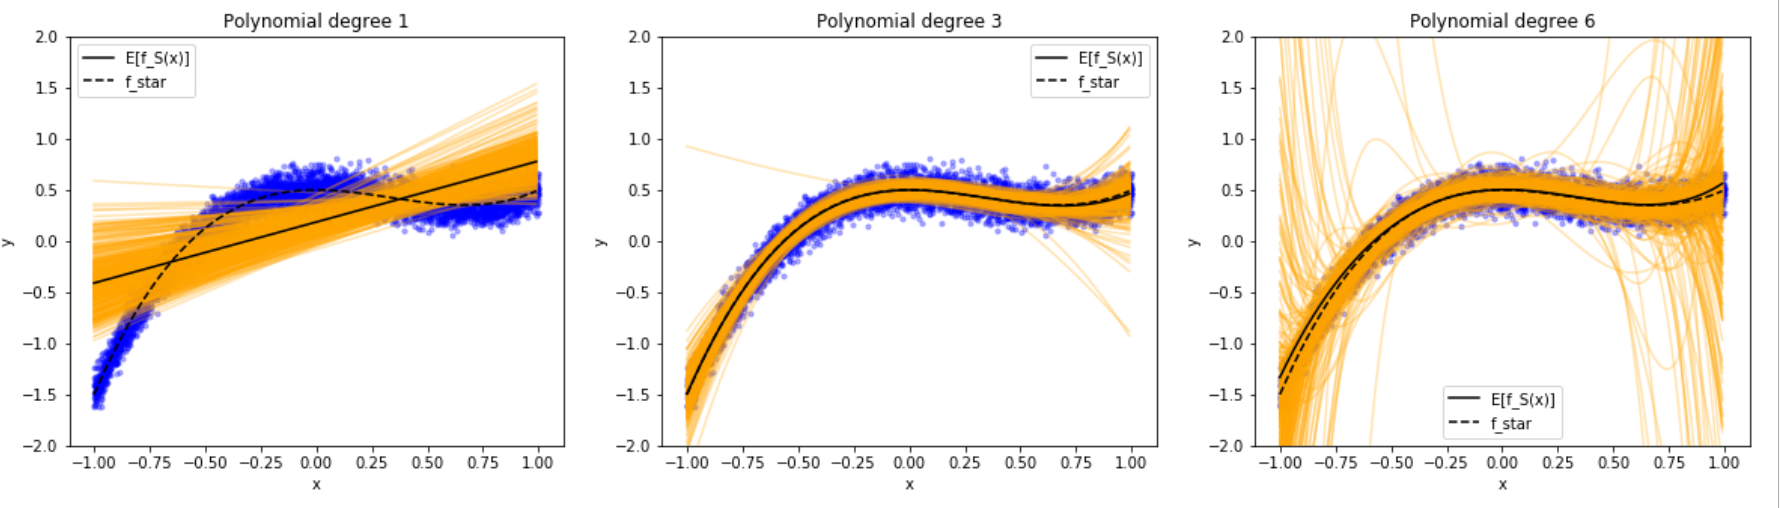
\includegraphics[width=17cm]{solution/bias_variance.png}\vspace{-2mm}
\caption{Visualizing the Bias-Variance Trade-off.}
\label{fig:bias_variance}
\end{figure}

\end{document}